\chapter{Theoretical background}

This chapter presents an overview of the Standard Model (SM) of Particle Physics which describes the particle nature of visible matter in the universe and unifies the electromagnetic, weak and strong interactions. 
Since a complete account of this monumental achievement far exceeds the scope of this document, only aspects of the theory most relevant to the rest of the thesis will be introduced. 
Interested readers are invited to peruse classic texts on the subject for further details~\cite{Peskin_2018, Halzen_Martin_2016, Schwartz_2014}.

\section{The Standard Model of Particle Physics}

Elementary particles in the SM are typically grouped by their spin. 
There are three generations of spin-$\frac{1}{2}$ particles called fermions, several spin-$1$ gauge bosons which mediate their interaction, and a spin-$0$ Higgs boson to account for other particles' mass. 
Two types of fermions exist; the first is the leptons, which include the electron ($e$), the muon ($\mu$) and the tau lepton $(\tau)$, and their associated neutrinos, denoted $(\nu_e, \nu_{\mu}, \nu_{\tau})$. 
The second type consist of three generations of quarks, each consisting of a pair, namely up $(u)$ and down $(d)$, charm $(c)$ and strange (also sideways) $(s)$, and top $(t)$ and bottom $(b)$. 

With the exception of neutrinos, all SM fermions carry an electric charge and couple to the \textit{electromagnetic} field via the photon. Leptons carry integer charge $\pm1$, while quarks carry fractional charges $\mp\frac{1}{3}e$ and $\mp\frac{2}{3}e$. 

Unlike leptons, quarks also carry $SU(3)$ color charge and couple to the gluon field, just like electrically charged particles coupling to the electromagnetic field. 
The spin-$1$ gluon also carries color charges and mediate the strong force between quarks and other gluons. 
It is due to the strong interaction that quarks always appear in bound states of a pair or a triplet called hadron, of which the proton and the neutron are examples, despite having same-sign electric charges. 
The color changes of bound quarks in hadrons always cancels each other, so hadrons are color-neutral. 

All fermions participate in the weak interaction, mediated by the $W^{\pm}$ and the $Z$ bosons, and responsible for decays of the muon and the tau lepton to the electron, and of quarks to lighter quarks, the most well-known example of which in nuclear physics is $\beta$ decay, and the top quark decaying to the bottom quark in particle physics. 
Unlike the photon and the gluon, the weak vector bosons are massive particles, whose mass is bestowed upon them by the Higgs mechanism which gives rise to the Higgs boson. 
The discovery of the Higgs boson in 2012 grants the SM its completeness and self-consistency. 

\section{Electroweak symmetry breaking and the Higgs mechanism} \label{sect:Higgs-mechanism}
The standard model, the left-handed leptons transform as an $SU(2)$ doublet, and the right-handed leptons transform as an $SU(2)$ singlet. Their Lagrangian must be invariant a under corresponding generic transformation
\begin{equation}
    \label{eq:2.1}
    E_L \rightarrow e^{\frac{i}{2}\left( \alpha^a(x)\sigma^a + \beta(x) \right)}E_L, \quad E_R\rightarrow e^{i\beta(x)/2}E_R,
\end{equation}
where $\alpha^a(x)$ and $\beta(x)$ are arbitrary differentiable functions, and $\sigma^a$ the Pauli matrices. To account for lepton masses, a scalar field invariant under local $SU(2)\otimes U(1)$ transformation is introduced
\begin{equation}
    \label{eq:2.2}
    \phi=\begin{pmatrix}
        \phi^+ \\ \phi^-
    \end{pmatrix}, \quad \phi\rightarrow e^{\frac{i}{2}\left( \alpha^a(x)\sigma^a + \beta(x) \right)} \phi,
\end{equation}
from which its covariant derivative follows as
\begin{equation}
    \label{eq:2.3}
    D_{\mu} = \partial_{\mu} - i \frac{g_2}{2}W^a_{\mu} \sigma^a - i\frac{g_1}{2}B_{\mu},
\end{equation}
where $A^{a}_{\mu}$ and $B_{\mu}$ are the $SU(2)$ and $U(1)$ gauge bosons. The most general Lagrangian for a renormalizable scalar field respecting these symmetries can be written as
\begin{equation}
    \label{eq:2.4}
    \mathcal{L}_{\mathrm{Higgs}} = \abs{D_{\mu}}^2 + \mu^2\phi^{\dagger}\phi - \frac{\lambda}{2} (\phi^{\dagger}\phi)^2
\end{equation}
The configuration which minimizes the Higgs potential, assuming $\mu^2 >0$, is such that 
\begin{equation}
    \label{eq:2.5}
    \phi^{\dagger}\phi = \frac{\mu^2}{\lambda} = v^2.
\end{equation}
The number $v$ is known as the vacuum expectation value (VEV) of the Higgs field. Selecting the simplest configuration, and adding a fluctuation field around the minimum, we get
\begin{equation}
    \label{eq:2.6}
    \expval{\phi} = \frac{1}{\sqrt{2}}\begin{pmatrix}
        0 \\ v
    \end{pmatrix}, \quad \phi = \frac{1}{\sqrt{2}}\begin{pmatrix}
        0 \\ v + H(x)
    \end{pmatrix}
\end{equation}
and evaluating the kinetic term in \eqref{eq:2.4}, we obtain terms suggestive of the mass eigenstates of the electroweak bosons
\begin{equation}
    \label{eq:2.7}
    \abs{D_{\mu}\phi} ^2 = \frac{1}{2}(\partial_{\mu}H)^2 + \frac{g_2^2}{8}(v+H)^2\abs{W_{\mu}^1 + iW_{\mu}^2}^2 + \frac{1}{8}(v+H)^2\abs{g_2W_{\mu}^3-g_1B_{\mu}}^2.
\end{equation}
By defining the mass eigenstates as
\begin{equation}
    \label{eq:2.8}
    W^{\pm}_{\mu}= \frac{1}{\sqrt{2}}(W_{\mu}^1\mp iW_{\mu}^2), \quad Z_{\mu} = \frac{g_2W_{\mu}^3-g_1B_{\mu}}{\sqrt{g_1^2+g_2^2}}, \quad A_{\mu} = \frac{g_2W_{\mu}^3 + g_1B_{\mu}}{\sqrt{g_1^2+g_2^2}}
\end{equation}
and the corresponding masses as
\begin{equation}
    \label{eq:2.9}
    M_W = \frac{g_2v}{2}, \quad M_Z = \frac{v\sqrt{g_1^2+g_2^2}}{2}, \quad m_A = 0
\end{equation}
and writing \eqref{eq:2.7} as
\begin{equation}
    \label{eq:2.10}
    \abs{D_{\mu}\phi} ^2 = \frac{1}{2}(\partial_{\mu}H)^2 + M_W^2\left(1+\frac{H}{v}\right)^2W_{\mu}^{+}W^{\mu-} + \frac{M_Z^2}{2}\left(1+\frac{H}{v}\right)^2Z_{\mu}Z^{\mu} + \frac{M_A^2}{2}A_{\mu}A^{\mu},
\end{equation}
we ``create" mass for the vector bosons, while maintaining a massless photon. It is convenient to introduce the electroweak mixing angle $\theta_W$ such that
\begin{equation}
    \label{eq:2.11}
    \tan\theta_W = \frac{g_1}{g_2} \Rightarrow \cos\theta_W = \frac{m_W}{m_Z}, 
\end{equation}
and that
\begin{equation}
    \label{2.12}
    \begin{pmatrix}
        Z_{\mu} \\ A_{\mu}
    \end{pmatrix} = \begin{bmatrix}
        \cos\theta_W & -\sin\theta_W  \\ 
         \sin\theta_W & \cos\theta_W  
    \end{bmatrix} \begin{pmatrix}
        W_{\mu}^3 \\ B_{\mu}
    \end{pmatrix}.
\end{equation}
We can rewrite the covariant derivative in \eqref{eq:2.4} using the mass eigenstates
\begin{align}
\label{eq:2.13}
    D_{\mu} &= \partial_{\mu} - i\frac{g_2}{2}W_{\mu}^a\sigma^a - i\frac{g_1}{2}B_{\mu} \\
    &= \partial_{\mu} - \frac{ig_2}{\sqrt{2}}(W_{\mu}^+T^+ + W_{\mu}^-T^-) - i\frac{1}{\sqrt{g_1^2+g_2^2}}Z_{\mu} (g_2^2T^3 - g_1^2 Y) \\ 
    & \quad - i\frac{g_1g_2}{\sqrt{g_1^2+g_2^2}} A_{\mu}(T^3+Y)
\end{align}
where $T^a=\sigma^a/2$, $T^{\pm} = (T^1\pm iT^2)$, $Y$ a general $U(1)$ charge. Defining the coefficient of the electromagnetic interaction $e=\frac{g_1g_2}{\sqrt{g_1^2+g_2^2}}$, and the electric charge quantum number $Q=T^3+Y$, we retrieve a covariant derivative where the couplings of all electroweak bosons can be described by the familiar electric charge and the mixing angle
\beq
\label{eq:2.14}
D_{\mu} = \partial_{\mu} - \frac{ig_2}{\sqrt{2}}(W_{\mu}^+T^+ + W_{\mu}^-T^-) - \frac{ig_2}{\cos\theta_W}(T^3-\sin\theta_WQ^2) - ieA_{\mu}Q
\eeq
By spontaneously breaking the symmetry $SU(2)_L\times U(1)_Y\rightarrow U(1)_Q$, three Goldstone bosons (three degrees of freedom) are absorbed by the $W^{\pm}$ and $Z$ boson, making them massive. The remaining $U(1)_Q$ symmetry is unbroken, so its generator, the photon, remains massless.

Fermion mass is generated by treating the same scalar field $\phi$ and its isodoublet $\tilde{\phi} = i\sigma^2\phi*$. Take for example the first generation of fermion, introduce the $SU(2)_L\times U(1)_Y$ invariant Yukawa Lagrangian
\begin{equation}
    \label{eq:2.15}
    \mathcal{L}_F = -\lambda_e\bar{L}\phi e_R-\lambda_d\bar{Q}\phi d_R - \lambda_u \bar{Q} \tilde{\phi}u_R + h.c.,
\end{equation}
and repeat the same procedure, we get 
\begin{equation}
    \label{eq:2.16}
    \mathcal{L}_F = -\frac{1}{\sqrt{2}}\lambda_e(v+H)\bar{e}_Le_R + ...,
\end{equation}
and the fermion mass
\begin{equation}
    \label{eq:2.17}
    m_f = \frac{\lambda_f v}{\sqrt{2}}
\end{equation}

After symmetry breaking, the Higgs Lagrangian can be written as
\begin{equation}
    \label{eq:2.18}
    \mathcal{L}_H = \frac{1}{2}(\partial_{\mu} H)^2 - \lambda v^2H^2 - \lambda v H^2 - \frac{\lambda}{4}H^4,
\end{equation}
from which the Higgs boson mass reads 
\begin{equation}
    \label{eq:2.19}
    M_H^2 = 2\lambda v^2 = -2\mu^2.
\end{equation}
The triple and quartic terms give rise to the Higgs self-interaction vertices with coupling strength given in terms of its mass and VEV by 
\begin{equation}
    \label{eq:2.20}
    g_{HHH} = \frac{3M_H^2}{v}, \quad g_{HHHH} = \frac{3M_H^2}{v^2},
\end{equation}

The Higgs coupling to gauge bosons can easily be read from terms in \eqref{eq:2.10} following $M_V\left(1+\frac{H}{v}\right)^2,$
and hence,
\begin{equation}
    \label{eq:2.21}
    g_{HVV} = \frac{2M_V^2}{v}, \quad g_{HHVV} = \frac{2M_V^2}{v^2}.
\end{equation}
Similarly, the Higgs coupling to fermion is proportional to the fermion mass
\begin{equation}
    \label{eq:2.22}
    g_{Hff} = \frac{m_f}{v}
\end{equation}
In addition, the vacuum expectation value $v$ is fixed in terms of the Fermi constant $G_F$, experimentally determined from muon decay
\begin{equation}
    \label{eq:2.23}
    M_W = \frac{g_2v}{2}  = \left(\frac{\sqrt{2}g_2^2}{8G_F}\right)^{1/2} \Rightarrow v = \sqrt{\frac{1}{\sqrt{2}G_F}} \approx 246 \,\mathrm{GeV}.
\end{equation}

\section{Standard Model Higgs boson production and decay}
\label{sect:higgs-production}
From the Higgs coupling structures derived from \ref{sect:Higgs-mechanism}, we can examine the main production mechanisms of the Higgs boson in $pp$ collision at the LHC. Figure \ref{subfig:higgs-production-xs} shows the production cross sections of the SM Higgs boson during $pp$ collision at center-of-mass energy $\sqrt{s}=13$ TeV as a function of the Higgs mass. 
The most important production mechanisms include gluon-gluon fusion $(ggF)$, vector boson fusion $(qqH)$, associated production with a vector boson $VH,\,(V=W,Z)$, associated production with a pair of top (bottom) quarks $t\bar{t}H$ $(b\bar{b}H)$, and associated production with a single top quark $(tH)$.

\begin{figure}[h!]
    \begin{subfigure}[b]{0.48\textwidth}
        \centering
        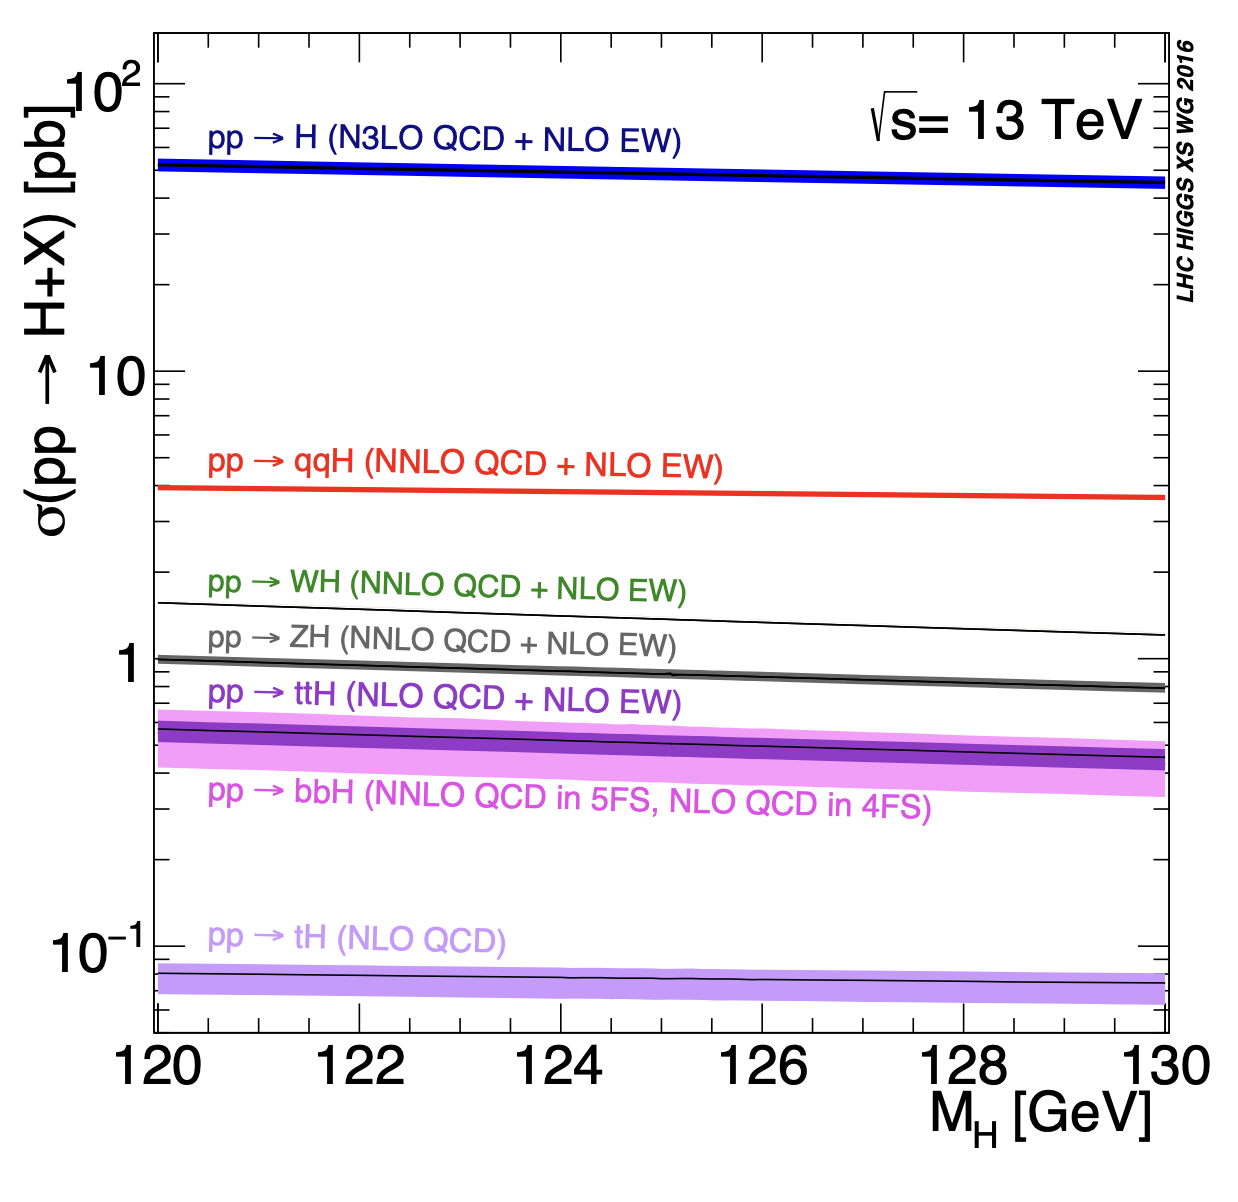
\includegraphics[width=\textwidth]{figures/higgs-xs.png}
        \caption{Production cross-section}
        \label{subfig:higgs-production-xs}
    \end{subfigure}
    \begin{subfigure}[b]{0.48\textwidth}
        \centering 
        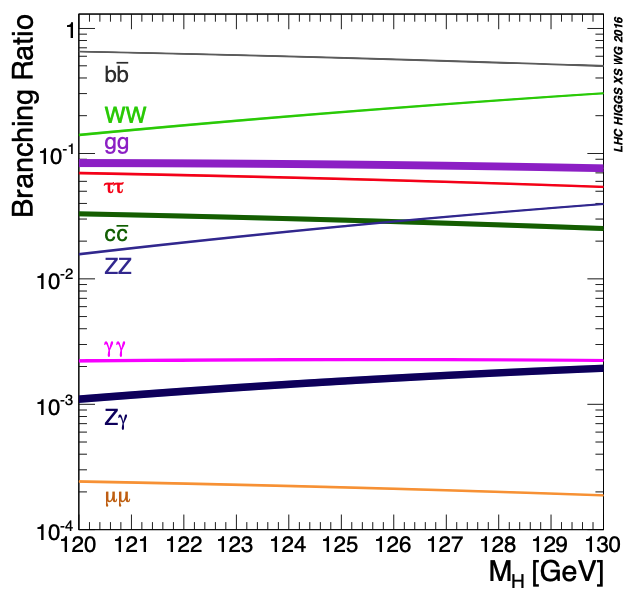
\includegraphics[width=\textwidth]{figures/higgs-branching-ratios.png}
        \caption{Branching ratio of Higgs decay}
        \label{subfig:higgs-br}
    \end{subfigure}
    \caption{Production cross-section of the Standard Model Higgs boson produced by $pp$ collision as a function of $M_H$ at $\sqrt{s}=13$ TeV}
    \label{fig:higgs-production-decay}
\end{figure}

The most dominant production mechanism is gluon-gluon fusion, whose cross-section far exceeds those of other mechanism. The Feynman diagram for this process is shown in figure \ref{subfig:gg-fusion-triangle}. The gluon is massless and only indirectly couples to the Higgs boson through a triangular heavy quark loop, to which the largest contribution comes from the top quark. The diagram still has a large magnitude, thanks to the strong coupling of the Higgs boson and the gluon to the top quark at this energy scale. 

Production via vector boson fusion $(VBF)$ sees the second largest cross-section, thanks to large couplings between the Higgs and the $W/Z$ bosons and between the vector bosons to heavy quarks, albeit an order of magnitude smaller than $\sigma_{ggF}$. Its tree-level diagram is shown in figure \ref{subfig:vbf}. The final state is characterized two forward jets from hadronized heavy quarks, along with products from various Higgs decay signatures. This process is particularly important in measurements of the $g_{HVV}$ coupling.

The leading diagram for associated Higgs production with a vector boson initiated by a pair of quarks $(qq\rightarrow VH)$ is shown in figure \ref{subfig:VH-higgs}. Another much smaller $gg$-initiated production also contribute at next-to-leading order. The Higgs boson is produced via Higgsstrahlungs from the vector boson. The letter can decay leptonically or hadronicall, but analyses in the leptonic channel often benefit from efficient lepton triggers, and high-quality lepton reconstruction. 

Finally, we mention the mechanism of associated production with a top quark pair, shown in figure \ref{subfig:ttH-signature}, which is small but of paramount importance in probing the Higgs coupling to the top quark. Unlike the case of other third-generation fermions, namely the tau lepton and the bottom quark, the Higgs decay to the top quark is kinematically forbidden due to the latter's large mass. Therefore, the top quark Yukawa coupling $y_t$ can only be measured through the $pp\rightarrow t\bar{t}H$ production process. 

\begin{figure}[h]
    \centering
    \begin{subfigure}[b]{0.48\textwidth}
        \centering
        \begin{tikzpicture}
          \begin{feynman}
            \vertex (t1) at (0,0);
            \vertex (t2) at (-0.866, 0.5);
            \vertex (t3) at (-0.866, -0.5);
            \vertex [above left = of t2] (a);
            \vertex [below left = of t3] (b);
            \vertex [right = of t1] (c);
            \diagram[horizontal = t1 to c] {
                (t1) -- [scalar, edge label=\(H\)] (c),
                (t1) -- [fermion, edge label=\({t}\)] (t3)  -- [fermion, edge label=\({t}\)] (t2) --[fermion, edge label=\({t}\)] (t1),
                (a) -- [gluon] (t2),
                (b) -- [gluon] (t3),
            };
          \end{feynman}
        \end{tikzpicture}
        \vfill
        \caption{Triangular gluon-gluon fusion production}
        \label{subfig:gg-fusion-triangle}
    \end{subfigure}
    \hfill
    \begin{subfigure}[b]{0.48\textwidth}
        \centering
        \begin{tikzpicture}
          \begin{feynman}
            \vertex (h) at (0.3,0);
            \vertex (tgp) at (-0.3, 1) ;
            \vertex (bgp) at (-0.3, -1) ;
            \vertex (gt) at (-1.8, 1.2) {$q$};
            \vertex (gb) at (-1.8, -1.2) {$q'$};
            \vertex (t) at (1.4, 1.2) {$q$} ;
            \vertex (b) at (1.4, -1.2) {$q'$};
            \vertex (htb) at (1.5, 0) {$H$};
            \diagram[] {
                (h) -- [photon, edge label = \($W/Z$\)] (tgp),
                (bgp) -- [photon, edge label = \($W/Z$\)] (h),
                (gt) -- [fermion] (tgp),
                (gb) -- [fermion] (bgp),
                (tgp) -- [fermion] (t),
                (bgp) -- [fermion] (b),
                (h) -- [scalar] (htb),
            };
          \end{feynman}
        \end{tikzpicture}
        \vfill
        \caption{Vector boson fusion production}
        \label{subfig:vbf}
    \end{subfigure}
    \vfill
    \begin{subfigure}[b]{0.48\textwidth}
        \centering
        \begin{tikzpicture}
          \begin{feynman}
            \vertex (t1) at (0,0);
            \vertex (t2) at (-0.7, 1.5) {$\bar{q}$};
            \vertex (t3) at (-0.7, -1.5) {$q$};
            \vertex (t4) at (2, 0.);
            \vertex (t5) at (2.7, 1.5) {$W/Z$};
            \vertex (t6) at (2.7, -1.5) {$H$} ;
            \diagram[] {
                (t1) -- [fermion] (t2),
                (t3) -- [fermion] (t1),
                (t1) -- [photon, edge label = \(W/Z\)] (t4),
                (t4) -- [photon] (t5),
                (t4) -- [scalar] (t6),
            };
          \end{feynman}
        \end{tikzpicture}
        \caption{Associated production with a vector boson}
        \label{subfig:VH-higgs}
    \end{subfigure}
    \begin{subfigure}[b]{0.48\textwidth}
        \centering
        \begin{tikzpicture}
          \begin{feynman}
            \vertex (h) at (0,0);
            \vertex (tgp) at (-0.3, 1) ;
            \vertex (bgp) at (-0.3, -1) ;
            \vertex (gt) at (-1.8, 1.2) {$g$};
            \vertex (gb) at (-1.8, -1.2) {$g$};
            \vertex (t) at (1.4, 1.2) {$q$} ;
            \vertex (b) at (1.4, -1.2) {$\bar{q}$};
            \vertex (htb) at (1.5, 0) {$H$} ;
            \diagram[] {
                (h) -- [fermion] (tgp),
                (bgp) -- [fermion] (h),
                (gt) -- [gluon] (tgp),
                (gb) -- [gluon] (bgp),
                (tgp) -- [fermion] (t),
                (b) -- [fermion] (bgp),
                (h) -- [scalar] (htb),
            };
          \end{feynman}
        \end{tikzpicture}
        \caption{Associated production with top quark pair}
        \label{subfig:ttH-signature}
    \end{subfigure}
    \caption{Leading-order Higgs boson production mechanisms}
    \label{fig:higgs-production}
\end{figure} 

Another consequence of the Higgs coupling structure described in \ref{sect:Higgs-mechanism} equally important to the study of the Higgs boson at the LHC is the consideration of its decay channels. 
Being one of the heaviest SM particles, the Higgs boson has a lifetime of approximately $10^{-22}s$. 
Tree-level Higgs boson decay is induced by its coupling to quarks, whose primary channels include $H\rightarrow b\bar{b}/c\bar{c}$, to leptons, namely $H\rightarrow \tau\bar{\tau}/\mu\bar{\mu}$, and to vector bosons, namely $H\rightarrow WW/ZZ$. 
In addition, notable loop-induced decays include $H\rightarrow gg/\gamma\gamma/Z\gamma$. Figure \ref{subfig:higgs-br} shows the branching ratios of primary Higgs decay channels as a function of the Higgs mass near $m_H=125$ GeV. Table \ref{tab:higgs-br} specifies the branching ratio measured at Higgs mass $M_H=125.09$ GeV.

\begin{table}[h]
    \centering
    \begin{tabular}{|l|c|}
    \hline \hline
     Decay channel    & Branching ratio $(\%)$ \\
     \hline
      $H\rightarrow b\bar{b}$   & $57.5\pm 1.9$ \\
      $H\rightarrow WW $   & $21.6\pm0.9$ \\
       $H\rightarrow gg$  & $8.56\pm0.86$ \\
        $H\rightarrow \tau\bar{\tau}$    & $6.30\pm 0.36$ \\
        $H\rightarrow c\bar{c}$    & $2.9\pm 0.35$ \\
        $H\rightarrow ZZ$    & $2.67\pm 0.11$ \\
        $H\rightarrow \gamma\gamma$    & $0.228\pm 0.011$ \\
        $H\rightarrow Z\gamma$    & $0.155\pm 0.014$ \\
        $H\rightarrow \mu\bar{\mu}$    & $0.022\pm 0.001$ \\
    \hline
    \end{tabular}
    \caption{Standard Model Higgs boson decay branching ratios and uncertainty at $M_H=125.09$ GeV}
    \label{tab:higgs-br}
\end{table}

Since a decay to the top quark is forbidden, it is not surprising that the most dominant decay mode is the $H\rightarrow b\bar{b}$ via Yukawa coupling, whose branching ratio is $57.5\%$ at $m_H=125.09$ GeV. 
Among other fermions, decay into a pair of tau leptons is the second largest, followed by decays into second-generation fermions (figure \ref{subfig:hff-decay}). 
The decay to a pair of vector boson proceeds through tree-level processes (figure \ref{subfig:hVV-decay}), whereas $H\rightarrow \gamma\gamma$ is mediated by a $W$ boson (figure \ref{subfig:hyy-W}) or a heavy quark loop (figure \ref{subfig:H-yy-t}). Despite having a small branching ratio, $H\rightarrow \gamma\gamma$ is an important channel for precision measurement of the Higgs mass due to the high resolution of the reconstructed photon invariant mass. 

\begin{figure}[h!]
    \centering
    \begin{subfigure}[b]{0.48\textwidth}
        \centering
        \begin{tikzpicture}
          \begin{feynman}
            \vertex (h) at (0,0) {$H$};
            \vertex [right = of h] (hff) ;
            \vertex [above right = of hff] (f1) {$b,\tau,c$};
            \vertex [below right = of hff] (f2) {$\bar{b}, \bar{\tau}, \bar{c}$};
            \diagram[horizontal = h to hff] {
                (h) -- [scalar] (hff),
                (hff) -- [fermion] (f1),
                (f2) -- [fermion] (hff),
            };
          \end{feynman}
        \end{tikzpicture}
        \vfill
        \caption{Higgs decay to fermions}
        \label{subfig:hff-decay}
    \end{subfigure}
    \hfill
    \begin{subfigure}[b]{0.48\textwidth}
        \centering
        \begin{tikzpicture}
          \begin{feynman}
            \vertex (h) at (0,0) {$H$};
            \vertex [right = of h] (hvv) ;
            \vertex [above right = of hvv] (v1) {$W/Z$};
            \vertex [below right = of hvv] (v2) {$W/Z$};
            \diagram[horizontal = h to hvv] {
                (h) -- [scalar] (hvv),
                (hvv) -- [photon] (v1),
                (hvv) -- [photon] (v2),
            };
          \end{feynman}
        \end{tikzpicture}
        \vfill
        \caption{Higgs decay to vector bosons}
        \label{subfig:hVV-decay}
    \end{subfigure}
    \vfill
    \begin{subfigure}[b]{0.48\textwidth}
        \centering
        \begin{tikzpicture}
          \begin{feynman}
            \vertex (h) at (0,0) {$H$};
            \vertex [right = of h] (hff) ;
            \vertex [above right = of hff] (f1) ;
            \vertex [below right = of hff] (f2) ;
            \vertex [right = of f1] (y1) {$\gamma$};
            \vertex [right = of f2] (y2) {$\gamma$};
            \diagram[horizontal = h to hff] {
                (h) -- [scalar] (hff),
                (hff) -- [fermion, edge label = \($t$\)] (f1) -- [fermion, edge label = \($t$\)]
                (f2) -- [fermion, edge label = \($t$\)] (hff),
                (f2) -- [photon] (y2),
                (f1) -- [photon] (y1),
            };
          \end{feynman}
        \end{tikzpicture}
        \caption{$H\rightarrow \gamma\gamma$ decays via $t$-loop}
        \label{subfig:H-yy-t}
    \end{subfigure}
    \begin{subfigure}[b]{0.48\textwidth}
        \centering
        \begin{tikzpicture}
          \begin{feynman}
            \vertex (h) at (0,0) {$H$};
            \vertex [right = of h] (hff) ;
            \vertex [above right = of hff] (f1) ;
            \vertex [below right = of hff] (f2) ;
            \vertex [right = of f1] (y1) {$\gamma$};
            \vertex [right = of f2] (y2) {$\gamma$};
            \diagram[horizontal = h to hff] {
                (h) -- [scalar] (hff),
                (hff) -- [photon, edge label = \($W$\)] (f1) -- [photon, edge label = \($W$\)]
                (f2) -- [photon, edge label = \($W$\)] (hff),
                (f2) -- [photon] (y2),
                (f1) -- [photon] (y1),
            };
          \end{feynman}
        \end{tikzpicture}
        \caption{$H\rightarrow \gamma\gamma$ decays via $W$-loop}
        \label{subfig:hyy-W}
    \end{subfigure}
    \caption{Leading-order Higgs boson decay mechanisms}
    \label{fig:higgs-decays}
\end{figure} 

\section{Extension of the Standard Model Higgs sector}
\label{sect:introduce-2HDM}

Until now, we have given a theoretical description of the simplest possible scalar structure of the Higgs field, namely a single $SU(2)$ doublet $\phi$. 
This assumption is motivated almost entirely by simplicity, and there exist a number of extensions to the SM Higgs sector which satisfy the experimental constraint on its scalar structure \cite{Zyla:2020zbs}. 
The simplest of such extensions consists of an additional scalar Higgs doublets--known as the two-Higgs-doublet model (2HDM). 

The model is motivated by several considerations, the best know of which is supersymmetry, which is explored in Ref. \cite{HABER198575}. Briefly speaking, supersymmetric quarks of charges $2/3$ and $-1/3$ cannot acquire their mass through coupling to a single Higgs doublet. Moreover, the cancellation of anomalies requires the existence of an additional Higgs doublet. Therefore, the Minimal Supersymmetric Standard Model (MSSM) must contain two Higgs doublets, as prescribed by the 2HDM.

In addition, while the SM cannot account for the baryon-antibaryon asymmetry of the early universe, the 2HDM, thanks to the flexibility of their scalar mass spectrum and additional sources of CP violation, can provide stronger theoretical explanation of this phenomenon. Aspects of electroweak baryogenesis in the 2HDM is explored in reference \cite{Joyce_1996, Funakubo_1994, Cline_1996, PhysRevD.55.3873, LAINE200123, LarsFromme_2006}. A comprehensive review of the rich phenomenology of the 2HDM can be found in Ref. \cite{Branco_2012}.

In the context of dark matter (DM) searches at the LHC, the 2HDM extended by a pseudo-scalar mediator $a$, denoted by \thdma, constitute an attractive benchmark model \cite{2HDMWGproxi}. The pseudo-scalar mediates the interactions between the visible sector of the 2HDM and the dark sector, assumed to include a single fermionic DM particle $\chi$. Chapter \ref{chap:combination-dark-matter-2hdma} presents a combination and summary of dark matter searches using $139\, \ifb$ of $pp$ collision data at $\sqrt{s}=13$ TeV collected by the ATLAS detector throughout LHC Run 2. 
Relevant phenomenological aspects of the \thdma are presented in \ref{sect:theoretical-considerations-2hdma}, along with important model parameters and experimental signatures to be examined by DM searches in ATLAS, many of which are introduced earlier in this chapter. 